\documentclass[10pt]{reportMaster}

\title{Recommender system for multiple online shops}
\author{S.\ Deckers}
\id{} %TODO find out id
\department{Artificial Intelligence}
\committee{Dr. K. Driessens \\ Dr. J. Derks}
\date{} %TODO fill in date of submission


% new line instead of indent for new paragraph
\usepackage[parfill]{parskip}
\usepackage{ dsfont }
\usepackage{amsmath}
\usepackage{textcomp} % for texttimes

% figure stuff
\usepackage{graphicx}
\usepackage{caption}
\usepackage{subcaption}


\begin{document}
\maketitle

%TODO add table of contents (be aware of numbering!)

%==============================================================
\chapter{Introduction}
Recommendation systems are systems that aim to make personalized content recommendations to its users.
They are widely used in the world wide web in different contexts such as movie recommendation in the streaming service Netflix or music recommendation as in last.fm as well as in e-commerce to recommend products that the user might purchase.
They seek to provide users with items that are new to them or they might not have discovered otherwise.

%Probelms with e-commerce data
While in the context of Netflix or last.fm the users actively search for new movies or music and intentionally use the recommendation system, in the context of e-commerce recommendations are usually shown while browsing the website.
This also reflects in the kind of input the users give to the recommendation system.
In systems like Netflix and last.fm the users give explicit feedback to different items in the form of ratings to express how much a user likes an item or by simply stating whether the user likes or dislikes an item.
E-commerce services in contrast need to derive user preferences from their purchase or browsing behaviour.
This kind of feedback is called implicit feedback.
For recommendation this kind of feedback leads to problems for several reasons.
First implicit feedback might be noisy, since it bases on the assumption that a user it interested in an item if he purchased it.
This assumption is not necessary true, because he may have bought it for a friend or is just unsatisfied with the product.
If a user watches a movie, he is able to give it a low rating.
This option is not necessarily available within online shops.
Moreover implicit e-commerce datasets do not contain any information about negative feedback.
Positive feedback, i.e. interest in a product, can be derived from purchases, shopping cart entries or page visits, but there is no indication for disinterest in an item.
While in a rating dataset items that are not liked by the user have a low rating and not rated ones are considered unknown, in e-commerce dataset it is unknown whether items that have not been purchased are not interesting or not known to the user.
This raises two problems.
It may happen that a user gets repeatedly recommendations of items he does not need, since he has no chance to mark them as interesting.
This might lead to decreased user satisfaction and recommendation performance, but this issue will not be addressed in the scope of this thesis.
The second problem is, that negative feedback is necessary for some recommendation models, since in general machine learning models cannot be trained if only instances of one class are available.
So some sampling techniques need to be investigated, to figure out how to treat unknown instances.

Moreover the available datasets vary in number of users, number of items and amount of sparseness.
The success of a specific recommendation technique depends on the available data.
So for a specific dataset a suitable recommendation algorithm need to be found. %TODO find reference to prove that different datasets need different techniques
In this thesis different algorithms will be investigated to find a suitable technique for product recommendation in e-commerce.
%TODO find a dataset with more items than users (I think in handbook was news dataset was mentioned)
%TODO add reference to further chapter where I will explain in more detail which techniques work well for which datasets

A general challenge for recommendation is the high dimensionality and sparseness of the data.
Usually there is a high amount of users and items, but a single user only interacts with a relatively small amount of items and many items are only considered by a small amount of users.
This must be taken into account for the choice of recommendation algorithms as well as for implementation aspects, especially for the representation of the large sparse matrix. %TODO ref to implementation section

%todo could add that there are interactive systems or configarionable ones
%todo also could add different requirements/criteria from the handbook


\section{Problem statement}
% Investigate different techniques, see how they perform, what are their pro and cons
The goal of this thesis is to find a recommendation system for e-commerce datasets.
It is required to provide accurate recommendations in terms of the precision measure described in section \ref{sec:eval} as well fast recommendation to preserve user satisfaction when using the online shops.
So the first tasks of this thesis is to implement different recommendation techniques, measure their performance on an e-commerce dataset and analyse their advantages and drawbacks.
The implemented techniques include different collaborative filtering approaches, i.e. memory-based and model-based collaborative filtering, and content-based recommendation, see section %TODO add ref to rs chapter
Some techniques, especially model-based collaborative filtering, need to be adjusted to the implicit feedback datasets, especially regarding the lack of negative feedback.
So a collaborative filtering algorithm is developed that learns latent factors from binary feedback by applying logistic regression.
To overcome the problems of missing negative feedback and the skewed data distribution as explained in section ... an AdaBoost approach is applied to the developed algorithm. %TODO add ref to section where i describe the data
%todo explain more detailed why I used AdaBoost

% How do they correlate, maybe hybrid
The single recommendation systems are evaluated and their errors are compared in order to find a hybrid technique that makes use of the benefits of different recommenders. %TODO add reference that shows that hybrids perform better
So the resulting recommendation lists are compared and investigated for correlation.
Techniques with low error correlation might be able to form a hybrid system with better results.


\section{Contribution}
% Comparative study of different algorithms for e-commerce data
There are three main contributions of this thesis.
First it serves as a comparative study of basic recommendation algorithms applied to a real e-commerce dataset.
Benefits and drawback are pointed out, especially concerning known problems with implicit feedback datasets.

% Logistic regression SVD
Second a new model-based collaborative filtering approach for binary data is suggested called \textit{LogRegSVD}.
It is an adaption of a common collaborative filtering approach based on singular value decomposition, adapted to binary data by incorporating logistic regression.

% AdaBoost for reco
Furthermore AdaBoost is applied to the presented algorithm to tackle some of the problems raising due to implicit feedback datasets.
AdaBoost was already applied to collaborative filtering by \cite{boostingCFRatings} on a rating dataset.
\cite{boostingAUC} applied it to implicit feedback datasets by optimizing ranking measures like the area under the curve (AUC) measure or the mean average precision (MAP, see \ref{sec:eval}).
This work is original in applying it to a logistic regression approach for recommendation on a real e-commerce dataset.


\section{Organization}
%TODO How is the thesis structured?






%==============================================================
\chapter{Related Work}
\label{sec:relatedWork}

\section{Recommender Systems}
\label{sec:recommenderSystems}
There are different types of recommendation systems.
They can be divided into collaborative filtering (CF), content-based (CB), demographic, knowledge-based or network-based recommenders. % TODO add reference
The most used ones are collaborative filtering and content-based recommenders.
These techniques are applied for the recommendation system developed in the scope of this thesis and will be addressed in the next two sections.
In section \ref{rs_others} the other mentioned techniques will be shortly introduced to complete the picture of possible recommendation techniques.

\subsection{Collaborative filtering}
\label{sec:collaborativeFiltering}
%TODO insert visible paragraph heads for different algorithms
%TODO emphasize formulas, make equations of important ones
\label{rs_cf}

\subsubsection{Memory-based collaborative filtering}
\label{sec:memBasedCF}
Collaborative filtering is the most implemented and successful recommendation technique. %TODO add reference
Recommendations are made based on the preferences of all users using their ratings in the context of Netflix or their purchases in an e-commerce context.
These information is represented as a matrix where users are represented as rows and columns represent the items.
Every matrix entry indicates the interaction of a specific user-item pair.
For e-commerce data there is an entry of 1 indicating preference for every item a user purchased.
The other entries remain empty or zero indicating that preference for these items are unknown. %todo maybe write an own chapter for data representation and put this there

Collaborative filtering techniques are divided again into two different approaches: memory-based and model-based approaches.
While memory-based approaches directly make use of the preference matrix, model-based approaches train an alternative model and use this model to make recommendations.
Model-based recommendation systems need some time to train the model, but are able to make faster recommendations, because it uses a more compact model instead of the full purchase matrix.
Moreover model-based techniques usually need less memory, because the full purchase matrix is not needed.

In this thesis two memory-based and one model-based approach were investigated.
The memory-based techniques are k-nearest-neighbour algorithms applied to the purchase matrix.
They either take the similarities between users or items into account. % TODO add references to other papers that use item-item approach
In the item-item approach those items are recommended that are closest to the items the current user has already purchased.
For every item $i$ the current user $u$ has not purchased a score is calculated by

\begin{equation}
	 S(u,i) = \sum_{j \in I(u)}{sim(R(:,i), R(:,j))}
\end{equation}

Here $R \in \mathds{R}^{n \times m}$ denotes the purchase matrix for $n$ users and $m$ items. $R(:,i)$ denotes the $i^{th}$ column vector. $I(u)$ is the set of items user u purchased.
Then those items are recommended that reach the highest score. %TODO add pseudocode algorithm
The function $sim(R(:,i), R(:,j))$ can be substituted by any vector similarity function.
In this thesis experiments were performed using cosine similarity or the Jaccard coefficient explained in section . %TODO write section and reference to it

The second memory-based algorithm is a user-user approach.
Here the similarities between users instead of items are taken into account.
In the first step the nearest neighbours of the current user $u$, denoted by $N(u)$, are determined by getting those users $v$ which reach the highest score according to

\begin{equation}
	S(u,v) = sim(R(u,:)^T, R(v, :)^T)
\end{equation}

$R(u,:)$ and $R(v,:)$ are the $u^{th}$ and $v^{th}$ row vectors of the purchase matrix, respectively.
The similarity function $sim(R(u,:)^T, R(v, :)^T)$ refers to the same vector similarities as in the item-item approach, see . %TODO add reference
After the nearest neighbours of user $u$ are obtained, those items are recommended that are purchased most often by the determined neighbours. %TODO add pseudo code algorithm

This approach is not able to guarantee a sufficiently large list of recommendations, if the neighbours $N(u)$ purchased less items than the number of required recommendations or additionally to those $u$ already purchased.
Being $I(N(u))$ the items the neighbours of $u$ purchased, a user-user approach is only able to recommend at most $|I(N(u)) \setminus I(u)|$ items to user $u$.
This may especially be a problem for users with only a few purchases, because the less items a user purchased the higher is the probability to find a user with the same set of purchased items.

%TODO move this to chapter with my work
%To reduce the chance of not being able to find a sufficiently large list of recommendations and ensure that there is at least one recommendation from the user's neighbours, only those neighbours are taken into account with a similarity score of less than 1, i.e. $S(u,v) = sim(u, v) < 1$, because a score of 1 means that $u$ and $v$ have purchased exactly the same set of items.

Another user-user approach that does not suffer from the above problem was implemented by ... %TODO find and add reference
Here for every item $i$ the current user $u$ has not purchased, the similarity score between the current user $u$ and every user who has purchased $i$ is calculated: 

\begin{equation}
	S(u,i) = \sum_{v \in U(i)}{sim(u,v)}
\end{equation}

The nearest neighbours are not directly determined, so the recommendations are not limited to the items the neighbours purchased.
The recommended items are those that were purchased by those users with the highest similarity to $u$.
%TODO run algorithm again and add to experiments

Both item-item and user-user perform on the full purchase matrix, but are expected to obtain different results.
While an item-item approach tends to recommend items with many common users who purchased them, a user-user approach works on user similarities.
Since item-similarities are not taken into account, i.e. items do not need many common users, recommendations with a user-user technique may generate more diverse recommendations.
For matrices like the purchase matrix in e-commerce datasets an item-item approach is supposed to obtain more accurate results, because the item-vectors are larger than the user-vectors and therefore are able to produce more confident similarities between them. 

Since memory-based approaches need to parse the whole matrix for every recommendation, these methods are quite slow in contrast to model-based approaches.
But they benefit from adaptivity, because they can immediately incorporate new purchases, and do not need to retrain a model after the purchase matrix is updated.
Moreover the results can be intuitively explained to the user, because these approaches simply bases on purchases of similar users or similar items.

\subsubsection{Model-based collaborative filtering}
\label{sec:modelBasedCF}
%Explain general svd %TODO add references
The most common model-based collaborative filtering approach works by matrix factorization like singular value decomposition (SVD).
It is aimed to find latent factor features to represent users and items instead of using the whole vectors from the purchase matrix.
Generally SVD decomposes a matrix $A \in \mathds{R}^{m \times n}$ into the matrices $U \in \mathds{R}^{m \times n}$, $\Sigma \in \mathds{R}^{n \times n}$ and $V \in \mathds{R}^{n \times n}$, such that 

\begin{equation}
	A = U \Sigma V^T
\end{equation}

The column vectors of $U$ are the eigenvectors of $AA^T$, the columns of $V$ are the eigenvectors of $A^TA$.
$\Sigma$ is a diagonal matrix $diag(\sigma_1, ..., \sigma_n)$ containing the square roots of the corresponding eigenvalues.  %todo explain relation to pca
The eigenvectors in $U$ and $V$ and their eigenvalues in $\Sigma$ are sorted such that $\sigma_1 \geq \sigma_i \geq ... \geq \sigma_n \geq 0$.
Intuitively $AA^T$ contains the similarities of row vectors, i.e. users.
Element $a_{ij}$ of $AA^T$ corresponds to the similarity between user $i$ and $j$, where user similarities are expressed as their common purchases.
The eigenvalues are stored in descending order of their eigenvalues in $U$ and span a vector space of the user similarities.
So the first column of $U$ is a vector pointing into the direction of highest user similarity. %TODO add svd reference
Item similarities are stored in V respectively.
Dimensions of the purchase matrix A can than be reduced by cutting lower eigenvalues in $\Sigma$ and their eigenvectors in $U$ and $V$, because the lower eigenvalues are less able to detect purchase patterns of different users or items and are therefore less able to derive user and item features from.
Cutting eigenvectors and eigenvalues up to $f \in \mathbf{R}$ results in the singular value decomposition 

\begin{equation}
	A_f = U_f \Sigma_f V_f^T
\end{equation}

with $A_f \in \mathds{R}^{m \times n}$, $U_f \in \mathbf{R}^{m \times f}$, $\Sigma_f \in \mathds{R}^{f \times f}$ and $V_f \in \mathds{R}^{n \times f}$.
This can be transformed to 

\begin{equation}
	A_f = U_f \Sigma_f^{1/2} \Sigma_f^{1/2} V_f^T = P_f Q_f
\end{equation}

with $\Sigma_f^{1/2} = diag(\sqrt{\sigma_1}, ..., \sqrt{\sigma_f})$, $P_f = U_f \Sigma_f^{1/2}$ and $Q_f = \Sigma_f^{1/2} V_f^T$.
Users and items are expressed as $f$ latent features in $P_f$ and $Q_f$ respectively.
So every user $u$ can be assigned a feature vector $p_u$ and every item $i$ a feature vector $q_i$, whose elements are from the same latent feature space.
Predictions are performed by multiplying these feature vectors.
Preference of user $u$ for item $i$ can be estimated by 

\begin{equation}
	\hat{r}_{ui} = p_u^T q_i
\end{equation}


%Explain linear regression approach commonly used for recommendation
There are several algorithms to compute a singular value decomposition like proposed in \cite{svdGolubSolution}.
For recommendation systems the reduced user and item representations are often trained by alternating least squares regression instead of applying numerical methods. %TODO add svd paper
For every user $u$ a feature vector $p_u \in \mathds{R}^f$ and for every item $i$ a feature vector $q_i \in \mathds{R}^f$ is learned by minimizing the cost function 

\begin{equation}
	\sum_{u, i}{(r_{ui} - p_u^T q_i)^2 + \lambda (||p_u||^2 + ||q_i||^2)}
\end{equation}

$e_{ui} = r_{ui} - p_u^T q_i$ is the error term that has to be reduced.
$\lambda (||p_u||^2 + ||q_i||^2)$ is a regularization term to prevent the model from overfitting.
Optimization is performed by gradient descent.
The feature vectors are updated into the opposite direction of the partial derivatives of the $p_u$ or $q_i$ vectors of the cost function.
This yields the update rules

\begin{equation}
	p_u = p_u + \alpha \sum_{ui}{e_{ui} q_i + \lambda p_u}
\end{equation}
\begin{equation}
	q_i = q_i + \alpha \sum_{ui}{e_{ui} p_u + \lambda q_i}
\end{equation}

where $\alpha$ denotes the learning rate.
This approach is referred to as batch gradient descent, because for every feature update an iteration over the whole training set is needed.
A faster way is stochastic gradient descent. %TODO add refernce to any paper that uses "my" version of stochatic descent
There a feature vector is updated for every trainings example what leads to update rules 

\begin{equation}
	p_u = p_u + \alpha (e_{ui} q_i + \lambda p_u)
\end{equation}
\begin{equation}
	q_i = q_i + \alpha (e_{ui} p_u + \lambda q_i)
\end{equation}
%todo explain difference between funk and me and why his methods doesn't work for me

% Sampling 
This approach is usually applied to rating datasets and raises some problems when applied to implicit feedback data.
While for rating data there are positive as well as negative preferences available in the form of different ratings, in e-commerce there are only purchased items to be considered at interesting for the user and not purchased items that may be either not interesting or unknown to the user.
The least-squares regression model cannot be trained only on the positive values, so some of the unknown instances have to be used for training as well.
In \cite{occf} different sampling and weighting methods are investigated to address this issue.
Here the negative training instances are obtained by randomly choosing them from the unknown instances.
For every positive user-item-pair $(u, i)$ two negative user-item-pairs $(v, i)$ and $(u,j)$, with $\{u, v\} \in U$ and $\{i, j\} \in I$, are chosen, such that user or items with many positive examples (i.e. many purchases) get about as many negative ones for ensure balanced classification problems. %TODO somewhere introduce U as set of Users and I as set of Items
To express uncertainty of the negative instances a weight $w_n$ is added to the feature updates as suggested in \cite{occf}, such that the update rules become $p_u = p_u + w_n \alpha (e_{ui} q_i + \lambda p_u)$ and $q_i = q_i + w_n \alpha (e_{ui} p_u + \lambda q_i)$. %todo try different weights for p_u and q_i maybe? 
The weight is set to $w_n = 1$ for known positive trainings instances and to $w_n < 1$ for the other randomly chosen negative weights. %TODO which weight is used? Add experiments and reference to it

%todo Add other approaches of sampling i have tried aman or one random value per positive training instance
%todo add other weighting schemes i have tried (user based from occf paper)


%todo what problems still arise and how do i solve them? (reference to boosting chapter)

%TODO add that tv show cf for collaborative filtering approach

\subsection{Content-based recommendation systems} %TODO see how content-based is written
\label{rs_cb}
%TODO write contentbased section
Another common approach is content-based filtering.
This approach generates recommendations from any kind of content-based item features independently from other users' preferences.
The item features may be information about genres, actors or directors in a movie recommendation context.
For the dataset used in this thesis there are categories and description texts about the items.
An item can be in multiple categories, so they are represented as vectors $\vec{x} \in \mathds{R}^{|C|}$ where $|C|$ is the number of available categories.
The vector elements $x_c \in \{0,1\}$ indicate whether the item belongs to a specific category or not. 
Texts are represented as word vectors $\vec{x} \in \mathds{R}^{|T|}$ with $T$ being the total number of words in any of the item descriptions.
The vector elements $x_i$ are either binary values indicating the occurrence or absence of a word in the text, the number of occurrences of a word (bag-of-word model) or the corresponding tf-idf value. %TODO explain tf-idf and the formula I used

% What algorithms can be applied? explain naive bayes (because it seems to be often used) and nearest neighbor (because of simplicity)
The general idea is to recommend items that are most similar to the items the user has already purchased with respect to the given content-based features.
Two algorithms have been implemented: Naive Bayes classification and k-nearest-neighbour. % TODO add bayes references
Naive Bayes determines the probability that a user purchases a specific item based on the likelihood of its single features.
For every user a profile is trained consisting of the prior probability that $u$ purchases an item $p_u(c=1)$ and  the likelihoods of $f$ item features $p_u(x_f|c=1)$.
The probability of $u$ purchasing an item given in terms of item features $x$ can be calculated using the Bayes theorem by 

\begin{equation}
\label{BayesPost}
	p_u(c=1|x) = \frac{p_u(c=1) p_u(x|c=1)}{p_u(x)+2} \propto \frac{p_u(x|c=1)}{p_u(x)+2}
\end{equation}

$p_u(c=1)$ denotes the probability that user $u$ purchases an item independently from its features.
This value is the same for any item, so for calculating the recommendations it can be left out.
$p_u(x|c=1)$ is calculated by 

\begin{equation}
\label{BayesEvid}
p_u(x|c=1) = \prod_f{p_u(x_f|c=1)+1}
\end{equation}
%TODO define p_u(x_f)|c=1)
due to the independence assumption.
The $p_u(x_f|c=1)$ are obtained by counting the number of items $u$ purchased that contain feature $x_f$ divided by the total number of features $u$ purchased.
The constants $2$ and $1$ in equations \ref{BayesPost} and \ref{BayesEvid} respectively are added to avoid that the probability becomes zero when one of the feature likelihoods is zero, i.e. when a user has not purchased an item of a specific feature.
This technique is called Laplace-smoothing. %TODO add reference

The second algorithm is another k-nearest-neighbour implementation similar to item-item approach explained in section \ref{sec:collaborativeFiltering}.
This is the same implementation as in the collaborative filtering recommendation system, but instead of the column vectors of the purchase matrix the category or text feature vectors are used.
In the case of bag-of-words or tf-idf representation of items the cosine-similarity is used.
For the binary text or category representation either cosine similarity or the Jaccard coefficient can be used.

The naive Bayes and the k-nearest-neighbour recommenders are expected to produce different recommendations, because with k-nearest-neighbour an item is likely to be recommended if its whole set of features is similar to the those of items the user has already purchased.
Naive Bayes in contrast also may recommend items that have single item features in common to many of the users purchases.

Content-based recommendation systems generate intuitive recommendations, since they are always similar to the items the current user already purchased.
But this also limits the recommendation to a specific set of items features, while in collaborative filtering a greater diversity of items can be recommended.
In e-commerce datasets this constraint may even be a problem, because recommendations that are too similar to the items a user already purchased may be useless to him.
For example if the recommendations only differ in size, colour or brand from the product the user already owns.
So for online-shops content-based recommender systems may only be used for new users or in combination with another collaborative filtering recommendation system. %TODO refer to hybrid chapter 

%TODO add pseudo code algorihtms for both approaches

 
\subsection{Other recommendation systems}
\label{rs_others}
%TODO write other rs section and find papers of implementations
% demographic and network recommenders.
Besides collaborative filtering and content-based recommendation there are other recommendation systems like knowledge-based, demographic or network recommendation systems.
Knowledge-based recommender systems are based on any kind of knowledge-base that has to be built and maintained by domain experts.

%TODO why are those systems not used here?

\subsection{Hybrid recommendation systems}
% shortly describe other hybrid sections from burke and why are they not used in this thesiss

%TODO explain switching hybrids

%TODO explain weighted hybrid

%TODO explain cascade hybrid 

%TODO explain other hybrids 


%==============================================================
\section{Boosting}
Boosting is an ensemble learning technique for classification that aims to improve the performance of a learning algorithms by training multiple models.
First boosting algorithms were introduced by Schapire \cite{boostingSchapire} and Freund \cite{boostingFreund}.
The idea is to train multiple models of the same type iteratively such that every model performs slightly better than the preceding model.
So even if the initial model is weak and only makes slightly better predictions than random guessing, boosting is able to train a strong classifier.
This is achieved by focusing on training instances that are hard to classify.
After a model $M_i$ is trained, the next model $M_{i+1}$ is trained with higher emphasize on trainings examples that are misclassified by $M_i$. 
When all models are trained predictions are made by majority voting of all trained models.

\subsection{AdaBoost}
The most known boosting algorithm is AdaBoost (adaptive Boosting) developed by Freund and Schapire (\cite{boostingIntro}).
Given a set of training instances $X = \{x_1, ..., x_n\}$ and their corresponding class labels $Y = \{y_1, ..., y_n\}$, with $y_i \in \{-1, 1\}$ the first model $M_1$ is trained on a sample set according to a distribution $D_1(i) = \frac{1}{n}$, so each training instance has the same probability of being added to the training set for the first model.
Sampling is performed without replacement, so in general one instance may occur more than once in the training set.
The model $M_t$ is then tested on the training set and the error $\epsilon_t$ is calculated as the amount of incorrectly classified instances.
Dependent on this error the model is assigned a weight $\alpha_t = \frac{1}{2} ln(\frac{1 - \epsilon_t}{\epsilon_t})$, such that better models have a higher impact on final predictions.
The model error is also used to build the distribution for the next model: 

$ D_{t+1}(i) = \frac{D_t(i)}{Z_t} \times 
\begin{cases}
	e^{-\alpha_t} & \text{if $ x_i $ was correctly classified} \\ 
	e^{\alpha_t} & \text{if $ x_i $ was misclassified}
\end{cases}
$

$Z_t$ is a normalization factor to ensure $D_{t+1}$ is a distribution.
For the next model $D_{t+1}$ misclassified training instances get a higher probability of being added to the training set, while correctly classified one get a more unlikely to be chose.
So the next model set higher emphasize on instances that are hard to classify.

In the final prediction all models participate according to their corresponding weights with $H(x) = sign(\sum_{t = 1}^T\alpha_th_t(x))$.


\subsection{Reweighting and resampling}
In the original AdaBoost approach explained in the last section the weights of the training instances are used for resampling.
So only a sample of the full available training set is used for one iteration and the weights correspond to the chance that a training instance is added to it.
Another approach is to incorporate the weights into the training process if it is possible in the used algorithm.
When AdaBoost is applied with reweighting in each iteration the whole training set can be used as usual.
A comparative study was performed in \cite{resamplingReweighting} showing that there is no remarkable difference in performance comparing reweighting and resampling.


\subsection{AdaBoost for recommendation}
Attempts were made using AdaBoost for recommendation among others in \cite{boostingCFRatings} and \cite{boostingAUC}.
AdaBoost is applied to the SVD - approach similar to the one explained in section \ref{rs_cf}.
In \cite{boostingCFRatings} is applied to a movie rating dataset by optimizing the mean squared error. %TODO check, what they optimized
In \cite{boostingAUC} AdaBoost was applied to an implicit feedback dataset, but instead of optimizing the prediction error, as it was attempted in this thesis, they optimized the ranking measures MAP and AUC (Area Under Curve) directly.
AUC is another measure to evaluate the precision of ranked lists taking also recall into account. %todo explain AUC  %TODO what dataset did they use? % TODO why don't I use this approach?
There the authors evaluated their approach on a movie rating dataset that they transformed into a binary feedback dataset.











%==============================================================
\chapter{Recommendation in e-commerce}
\label{sec:ecommerceRec}
Different approaches from the last chapter were implemented and applied to a e-commerce dataset.
In section \ref{sec:comparison} the basic approach are analysed and compared.
Some enhancements were made with respect to e-commerce datasets, described in sections \ref{sec:logRegSVD} and \ref{sec:myAdaBoost}.


\section{Comparison of basic approaches}
\label{sec:comparison}
%TODO What and how did I implement?
Basic approaches explained in section \ref{sec:recommenderSystems} are implemented and analysed on how suitable they are for e-commerce.
Both an item-item and a user-user approach like described in section \ref{sec:memBasedCF} are implemented.
The item-item approach from ... was directly implemented without any changes. %TODO ref to algorithm
The user-user algorithm from ... was used. %TODO add ref to algorithm and explain why I did not use the other one
As in many applications the cosine similarity is used for both approaches.
Since the user and item vectors are binary experiments were also performed using Jaccard similarity. %TODO explain why Jaccard sim is supposed to perform better

The collaborative filtering approaches cannot be applied directly to implicit feedback datasets.
%TODO continue



\section{Matrix factorization using logistic regression}
\label{sec:logRegSVD}
%TODO 
%TODO move to my work chapter
%Explain my adaption to logistic regression
In most applications of this CF-approach, the user feedback $r_{ui}$ is given as any kind of explicitly given rating.
This information is not available in the e-commerce datasets, but there is information about whether a user purchased an item.
This yields binary values for $r_ui$, where $r_{ui} = 1$ denotes that user $u$ has purchased item $i$, and $r_{ui} = 0$ denotes that he has not.
So predicting user preferences becomes a classification rather than a regression problem.
So in the scope of this thesis the SVD approach is transformed into a logistic regression problem trying to predict a value $r_{ui} \in {0,1}$.
Prediction is performed by $\hat{r}_{ui} = \frac{1}{1 + e^{-p_u^Tq_i}}$.
When training the updates of user and item features vectors the prediction error is then replaced with $e_{ui} = r_{ui} - \frac{1}{1 + e^{-p_u^Tq_i}}$.
%todo add experiments to compare linear and logistic regression with lara

\section{AdaBoost}
\label{sec:myAdaBoost}
%TODO How did I apply AdaBoost
Here boosting was applied to the logistic regression algorithm for training the SVD model.

%TODO explain the used algorithm

%TODO how did I update the weights?

%TODO why did I use reweighting?

%TODO how prediction is made

%TODO apply userbased and articlebased prediction

%TODO add pseudocode













%==============================================================
\chapter{Implementation and Performance}
%TODO write implementation and performance chapter introduction

\section{Reactive design}
%TODO write reactive design section

\section{Implementation of purchase matrix}
%TODO write purchase matrix implementation section

\section{Architecture}
%TODO write high level architecture section

%TODO maybe add results for different matrix implementations







%==============================================================
\chapter{Experimentation}
The described algorithms are evaluated against a sample e-commerce dataset.
On one hand it is aimed to compare different recommendation approaches on e-commerce data and on the other hand the impact of different parameters is analysed to be able to tune algorithms for different datasets.
In the next section the data used for evaluating the algorithm is presented.
\ref{sec:eval} explains the used evaluation measures.
The last two sections of this chapter show the obtained results and discuss them.

\section{Data}
%TODO write data section
To evaluate the different recommendation approaches data from an online pharmacy is used.
The dataset contains purchases from 81835 users and 14964 articles.
Those n' articles contain many duplicates, because article of the same product, but with different package sizes or different colours are considered as different articles in the database.
There is no attribute to determine real distinct articles, but the amount of duplicates could be reduced by aggregating items of the same name and handle them as one item.
This reduces the number of items to 11775.
So dimensions of the used purchase matrix are 81835 \texttimes \ 11775.
It contains 663731 purchases, so it is only 0.06888\% dense, there are on average 56.37 purchases per item and 8.11 purchases per user. % TODO make table out of stats
Figure \ref{fig:dataDistribution} shows a histogram showing how the purchases per user and item are distributed.

%todo add median, 1st and 3rd quantile and create boxplots

%TODO make nicer plot (with visible axis labels...)
\begin{figure}
	\label{fig:dataDistribution}
	\begin{subfigure}[c]{1\textwidth}
		\caption{Distribution of user purchases.}
		\centering
		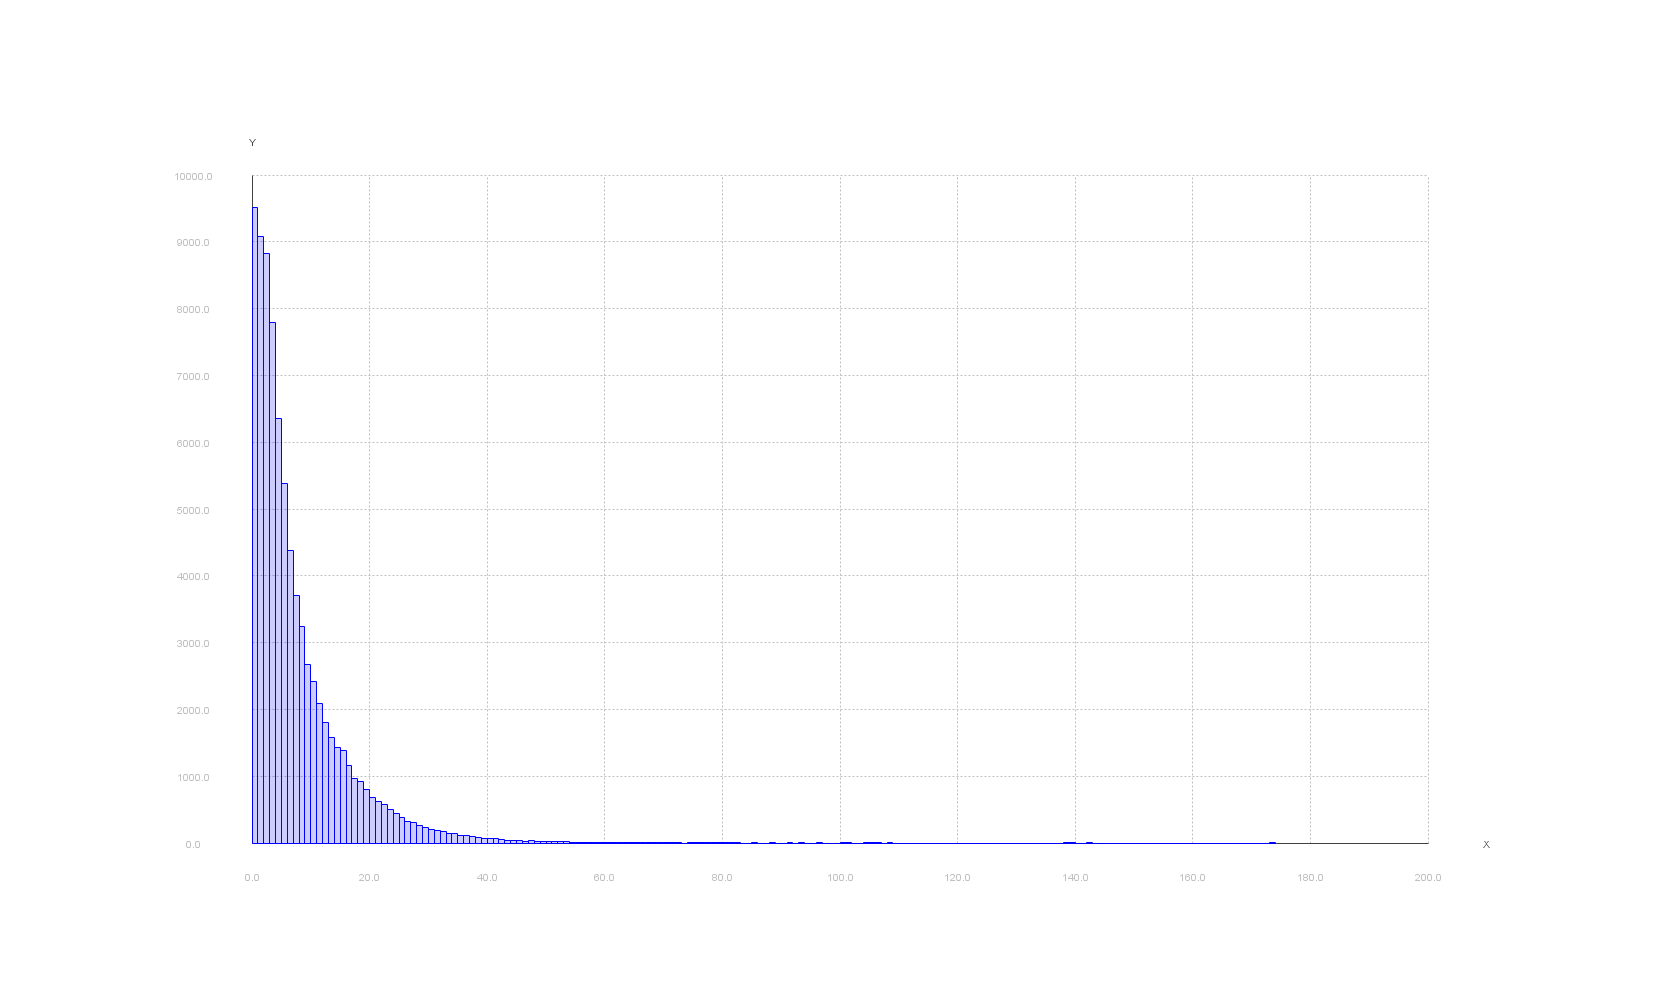
\includegraphics[width=1\textwidth]{figures/experiments/userPurchaseHistogram}
	\end{subfigure}
	\begin{subfigure}[c]{1\textwidth}
		\caption{Distribution of article purchases.}
		\centering
		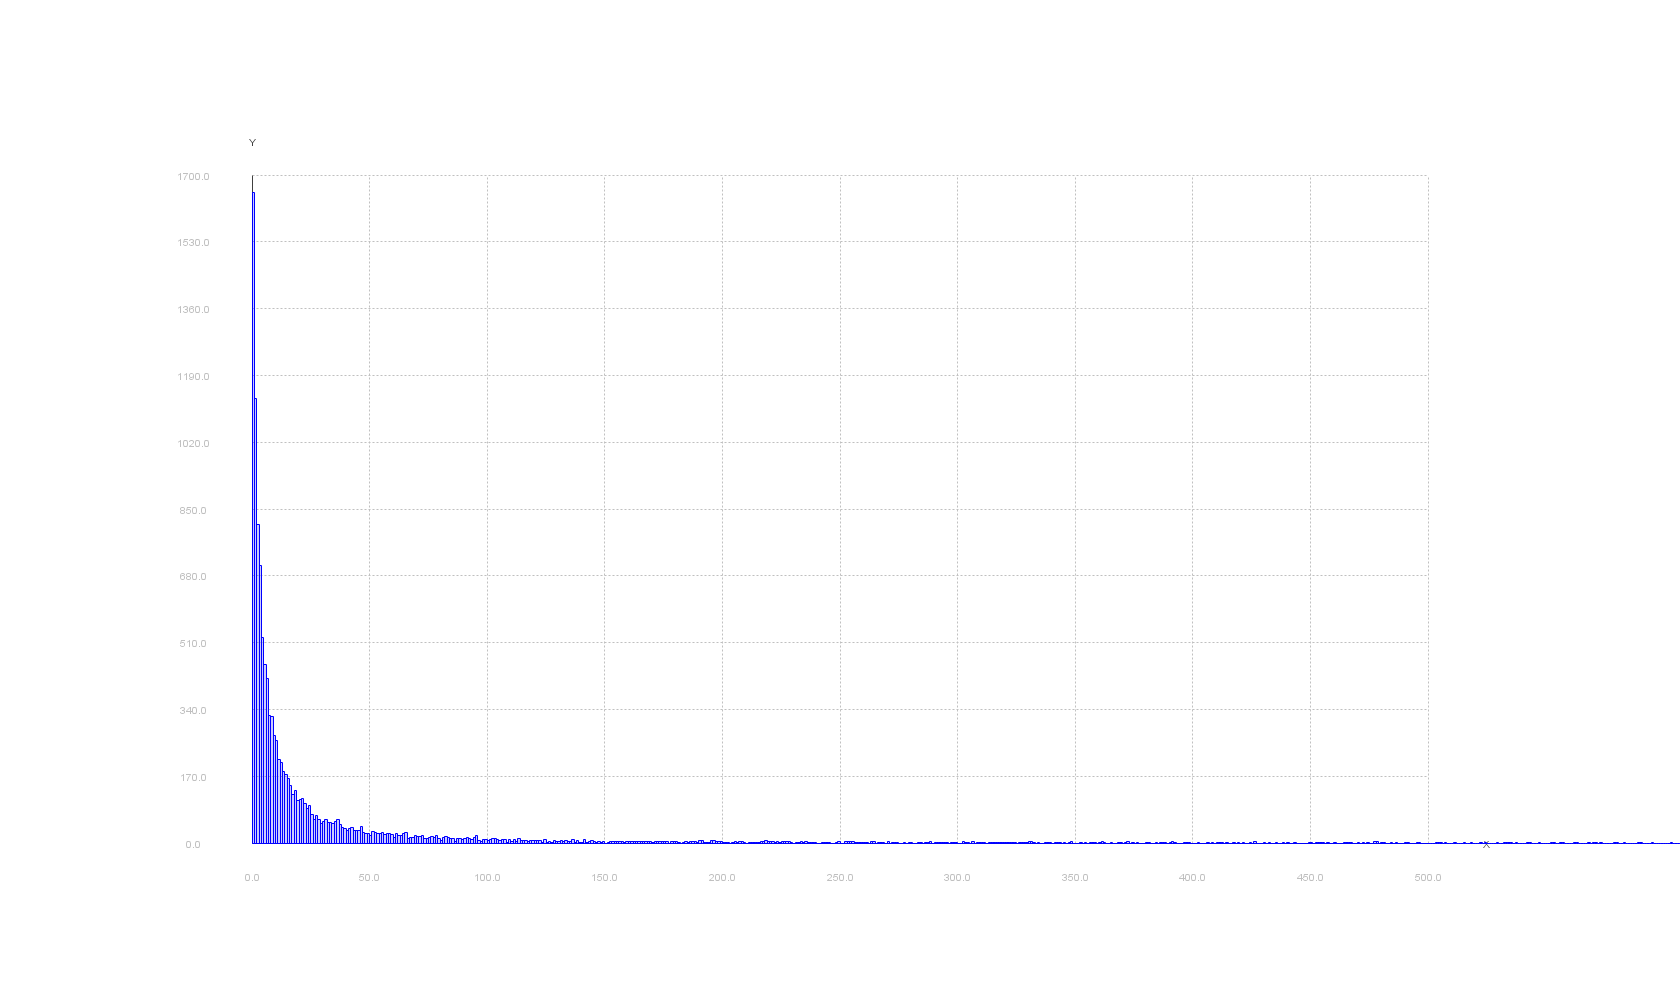
\includegraphics[width=1\textwidth]{figures/experiments/articlePurchaseHistogram_partly}
	\end{subfigure}
	
\end{figure}

Besides purchases there is content-based information about items.
Most items are assigned one or more categories they belong to.
Moreover there are different kinds of texts like descriptions, content or usage information.

%todo Eventually demographic information and other browsing history stuff


\section{Evaluation}
\label{sec:eval}
The recommendation systems are evaluated using 80 percent of the data as training set to treat as given and to build the model and 20 percent as test set.
The test set is built by iterating user- and item-wise over purchases and adding every 5th item to the test set and removing it from the training set.
This ensures that the test purchases are equally distributed over all users.
Users that only have purchased one item, are removed beforehand, because they cannot be evaluated, since at least one item must be left for training.
Users with no purchase are so called cold-start users and require another unpersonalized recommendation technique.
%TODO what are dimension of used dataset? what training and test sets?

Cold-start users are not of interest in this thesis, but an unpersonalized recommendation technique is used as a baseline for evaluation.
This used approach is denoted \textit{MostPop} and always recommends those items to a user that are purchased most often and were not yet purchased by the current user.

Evaluation is measured in terms of the mean average precision, a common measure in information retrieval.
It is a measure for evaluating ranked list, since it measures precision and incorporates the rank of correct recommendations.
It is calculated by:

\begin{equation}
	MAP_n = \frac{1}{|U|} \sum_u^{|U|} \frac{1}{|I_u|}\sum_i^{|I_u|} Precision(i)
\end{equation}

Here $U$ is the set of users who got recommendation in the evaluation process and $I_u$ is the list of items that is recommended to user $u$.
$Precision(i)$ denotes the precision of the recommended list up to position $i$, i.e. the number of correct recommendations within list elements $1$ to $i$ divided by $i$.
So it is the mean of precisions measured at every position of the list of recommendations averaged over all users who got recommendations.
All experiments are performed calculating a ranked list of ten recommendations.
Larger lists would increase performance, because more items would participate in the evaluation and could increase the precisions. %todo how large is the list in literature? difference in evaluation in contrast to rating predcition?
But in an online-shop a list of more than ten recommended items would not be useful to the user, since the recommended items are not actively requested by the user, but only shown besides the user browses the shop.
MAP is a good measure to evaluate the accuracy of a ranked list, but it is quite unintuitive.
So next to the MAP the precision independent of the rank is measured, i.e. how many of the test instances were recommended correctly, and the user precision is measured.
User precision means the amount of users who got at least one correct recommendation.


\section{Results}
The unpersonalized approach receives a MAP of 0.0499, a user precision of 0.2453 and an overall precision of 0.13142, i.e about 25\% of users got at least one correct recommendation and 13\% of items from the test set were correctly recommended to the users who purchased them.
The developed personalized recommendation systems are supposed to being able to outperform approach.

% How does CFItemNN perform with Jaccard and Cosine?
The model-based collaborative filtering approaches were evaluated using either the Jaccard coefficient or cosine similarity.
The item-item approach will further be denoted CFItemNN, while CFUserNN refers to the user-user approach.
CFItemNN works better using the Jaccard coefficient resulting in a MAP of 0.1371, a user precision of 0.3897 and an overall precision of 0.2269.
% TODO add cosine

%TODO How does CFUserNN perfrom with Jaccard and Cosine over number of neighbors?
CFUserNN was tested with the Jaccard coefficient and cosine similarity as well.
Moreover the performance was measured over different neighbourhood sizes.
%TODO plot both curves (Jaccard and cosine) over neighborhood sizes
%mention best settings for each curve
%in discussion section: with increasing neighbors CFUserNN converges to MostPop

%TODO How does SVD perform over different number of iteration?


%TODO How does it perform over number of features?
%TODO How does it using different weights for negative weights?

%TODO Which prediction scheme for AdaBoost performs best?

%TODO How does does CBNN perform?
	% with categories using Jaccard and Cosine
	% with text using binary word representation using Jaccard and Cosine
	% with text using bag-of-words model using Cosine
	% with text using tf-idf model using Cosine
	
%TODO How does Naive Bayes perform?

%TODO How do results of different recommendation techniques correlate?

%TODO cascade using mostPop (using candidate with at least x purchases)

%TODO add summary/comparison of best performers for every algorithm, how much better is it than baseline (in percent)?

\section{Discussion}
% TODO wirte discussion intro

\subsection{Single recommendation systems}
%TODO Explain strong and weak performers. What are pros and cons.


\subsection{AdaBoost}
%TODO Why does AdaBoost improve results?
%TODO explain different perfomances of prediction schemes

\subsection{Hybrid recommendation systems}
%TODO why is a hybrid recommender not useful

%TODO why does cascade with mostPop work (at least for some thresholds)




%==============================================================
\chapter{Conclusion and Future Work}
%TODO write conclusion and future work




%TODO add tables of figures, equations, tables and abbreviations



\bibliography{thesis_report}
\bibliographystyle{unsrt}
\end{document}

